  \newpage
  \subsection{Create a new run}
Every Organizator can create a new run, specifing the start and finish locations, date, time and the maximum number of enrollments.

\begin{table}[H]
	\centering
    
    \begin{tabular}{|p{3.5cm}|p{10.3cm}|}
    
    \hline
    \textbf{\large{Actors}}  			& \tabitem Organizator 	\\
    				 					
    \hline
    \textbf{\large{Goals}} 				& \ref{goal:run1}\\
    
    \hline
    \textbf{\large{Enter Condition}}	& The Organizator is already logged in.		\\
    
    \hline
    \textbf{\large{Events Flow}}		& \begin{enumerate}[leftmargin=0.5cm]
                                          	\item The \emph{Organizator}  accesses to the "Create Run" page of the application.
                                            \item The \emph{Organizator} inserts all the required informations to define the run (start and finish locations, date, time and maximum number of partecipants).
                                             \item The \emph{Organizator} defines the list of intermediate locations that will be part of the run's path.
                                            \item The System adds the new run into the list of scheduled runs.
                                           
                                          \end{enumerate}
    										\\
    \hline
    \textbf{\large{Exit Conditions}}    & The new run is created and successfully added into the list of scheduled runs.  \\
    
    \hline
    \textbf{\large{Exceptions}} 		& \begin{enumerate}[leftmargin=0.5cm]
                                          	\item The \emph{Organizator} specified a start or finish location that does not exist.
                                            \item The \emph{Organizator} specified intermediate points not reachable on foot.
                                             \item The \emph{Organizator} specified a negative maximum number of partecipants.
                                            \item The \emph{Organizator} specified a date or time that is already passed or the current day.
                                            \item The \emph{Organizator} specified a run with all the same informations of another run.
                                          \end{enumerate}
    										If one of these problems occur, the system shows an error message to the user, which is invited to re-insert the required informations for creating a new run.\\
    
    \hline
    
    \end{tabular}
	
\end{table}

\begin{figure}[H]
    \centering
    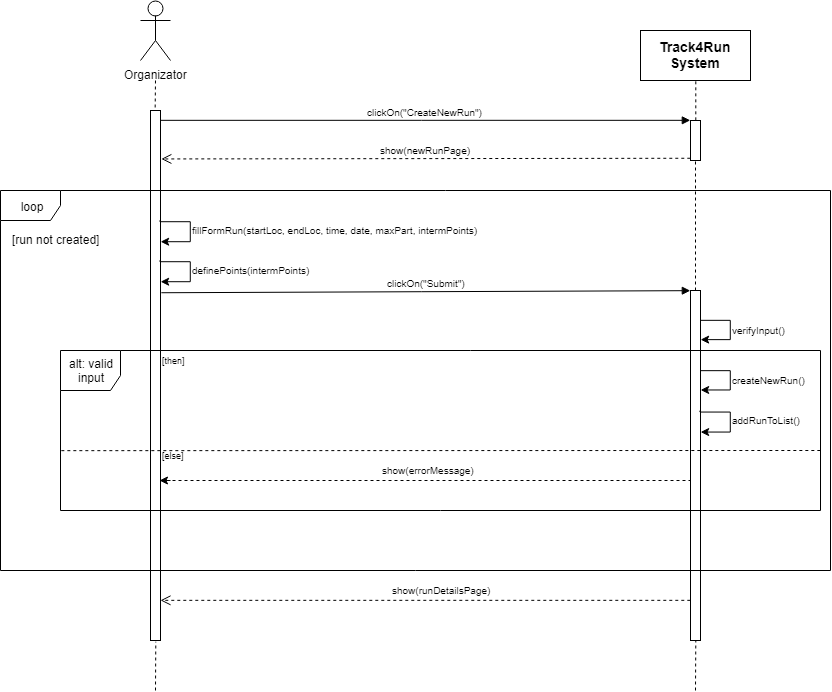
\includegraphics[scale=0.4]{Pictures/createNewRunSeqDiag.png}
    \caption{Sequence diagram for creating a new run}
\end{figure}
